\section{Benchmark NIST-4 "Peak"}
\label{sec:bench-4}

This problem has an exponential peak in the interior of the domain.
The equation solved in this benchmark problem is the Poisson's equation.

\begin{equation} \label{poisson-peak}
-\Delta u = f,
\end{equation}
in the domain $\Omega = (0, 1)^2$, equipped with Dirichlet
boundary conditions given by the exact solution.

The exact solution:
\begin{equation}\label{exact-nist-4}
u(x,y) = e^{-\alpha ((x - x_{loc})^{2} + (y - y_{loc})^{2})},
\end{equation}
where $(x_{loc}, y_{loc})$ is the location of the peak, and $\alpha$ determines the strength of the peak.
The right-hand side $f$ is calculated by inserting (\ref{exact-nist-4}) into (\ref{poisson-peak}).
The solution of NIST-4 with $\alpha = 1000$, $(x_{loc}, y_{loc}) = (0.5, 0.5)$ is shown in Fig. \ref{fig:sln-nist04}.

\begin{figure}[!ht]
\centering
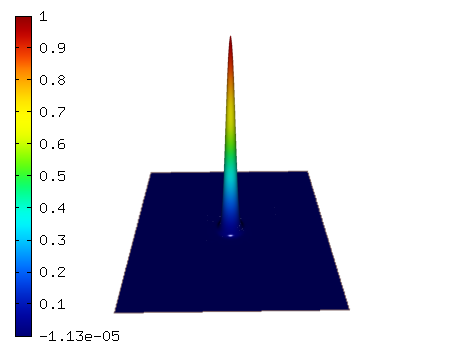
\includegraphics[height=5cm]{nist/nist-4/solution.png}
\caption{The solution to NIST-4 benchmark problem.}
\label{fig:sln-nist04}
\end{figure}
